\documentclass[11pt, conference]{IEEEtran}
\usepackage{amsmath, amssymb, amsfonts}
\usepackage{algorithmic}
\usepackage{graphicx}
\usepackage{textcomp}
\usepackage{xcolor}

\usepackage[figurename=Fig.]{caption}
\usepackage{subcaption}
\captionsetup[table]{labelsep=space}
\captionsetup[figure]{labelsep=period}

\usepackage{multirow}
\usepackage{booktabs}
\usepackage{cite}

\begin{document}
\title{Machine Learning Models for Mushroom Classification: Poisonous vs. Edible}
\author{
    \IEEEauthorblockN{Steven Alvarado}
    \IEEEauthorblockA{}
    \and
    \IEEEauthorblockN{Noor Ashour}
    \IEEEauthorblockA{}
    \and
    \IEEEauthorblockN{Khaiber Amin}
    \IEEEauthorblockA{}
    \and
    \IEEEauthorblockN{Dhruv Arora}
    \IEEEauthorblockA{}
}

\maketitle
\begin{abstract}
    The consumption of wild mushrooms poses inherent risks due to the potential presence of toxic species. Thus, accurate classification of mushroom edibility is crucial for ensuring the safety and efficiency of mushroom foraging. This report presents a comprehensive investigation into the efficacy of various machine learning models for classifying poisonous mushrooms based on physical attributes.
    
    With a dataset comprising morphological features of numerous mushroom species, we employ a range of machine learning algorithms including neural networks, decision trees, and random forests to classify mushrooms as poisonous or edible. Performance metrics such as accuracy, precision, recall, and F1 score are recorded to evaluate the models' classification abilities. Furthermore, feature importance analysis is conducted to discern the most influential attributes in the classification process. This aids in understanding the underlying characteristics that distinguish edible from poisonous mushrooms, contributing to both model interpretability and domain knowledge.
\end{abstract}

\section{Introduction}
    \subsection{Background}
    Valued for their nutritional and therapeutic benefits, mushrooms have long been a part of the human diet and possess a rich and distinct history as one of the world's staple food sources. One of the key benefits of mushroom foraging is the high nutritional value and unique flavors that these fungi can provide. However, not all mushrooms are deemed safe for human consumption, with certain species capable of causing severe illness or death at lethal doses. Many wild mushrooms have the potential to be poisonous, making proper identification crucial to avoiding potential harm. In the wild, assessing the edibility of a mushroom with the naked eye alone can be a time-consuming and error-prone process. With no simple tests or rules to remember, it takes extensive knowledge and experience to confidently identify species of mushrooms that are safe for ingestion.

    \subsection{Problem Statement}
    Therefore, our problem lies in finding a fast and reliable method for classifying a mushroom's edibility. Machine learning models can be trained to classify mushrooms based on their physical attributes, such as their odor, cap shape, ring type, gill size, etc. Our goal is to train and evaluate several of these classification models for their ability to accurately differentiate between poisonous and edible mushrooms. With this, we hope to optimize the safety and speed of mushroom foraging, where the best models can greatly reduce the risk of error and ultimately automate the identification process.
    
\section{Literature Review}
    To build a better understanding of how to approach this problem, background research was conducted to review any relevant and potential methods that already exist. Multiple published papers concerning the topic of mushroom identification were reviewed. Firstly, we researched the different methods used for mushroom classification. This included macroscopic, microscopic, and molecular identification techniques, as well as spectral and chromatographic methods [1]. Although each method has its advantages and disadvantages, we learned that macroscopic identification is the type of observation that our mushroom dataset is typically concerned with, where the physical attributes of the mushrooms are strictly examined. Our dataset consists of these naked-eye observations as our variables, such as cap shape, cap color, gill size, veil type, stalk shape, etc.
    
    Some peer-reviewed papers also inspired a plethora of different classification algorithms we can include in our experiments. Many of the studies we researched compared multiple algorithms and/or models to see which ones were the most effective. In “Classification algorithm for edible mushroom identification,” three different models are compared: Decision Tree, Naive Bayes, and Support Vector Machine [2]. This study also used the same data set that we will be using. In another study that we looked into, pre-trained (CNN) models were used, which included VGG16, ResNet50, and Inception V3 [3]. This study differs from ours in that it used images instead of macroscopic observations for the dataset. Based on these related papers, we followed the trend of comparing multiple models and gathering insight on which ones perform optimally. Ultimately, these studies inspired us to explore and compare a large range of models with a greater understanding of their implications in performance.

\section{Dataset Description}
    For this project, we use the "Mushroom" dataset from the UCI Machine Learning repository, containing 8,124 instances and 22 categorical features of gilled mushrooms in the Agaricus and Lepiota families. A corresponding dataset can be found on Kaggle with a formatted CSV file of the mushroom samples. Both of these resources were utilized to help form a complete understanding of our model implementation. Imported from the UCI repo, included with the dataset is a file named "agaricus-lepiota.names", which is a brief collection of notes provided by the dataset donor. Some of these comments helped us format the data during the exploratory data analysis phase, particularly for missing values found in the stalk root feature.

    % Figure 1: Mushroom features
    \begin{figure*}[ht!]
        \centering
        \subfloat[Cap shape.]{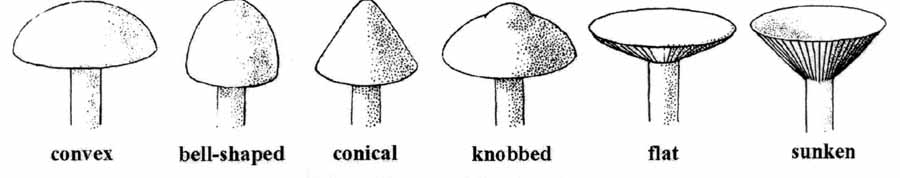
\includegraphics[width=0.5\textwidth]{plot/graphic/cap shape.jpg}}
        \subfloat[Cap surface.]{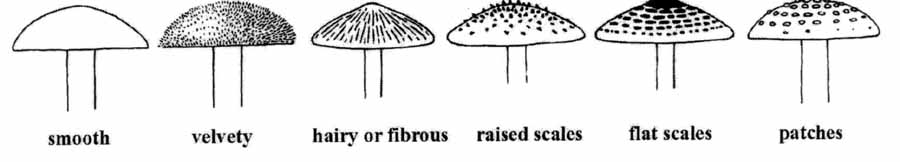
\includegraphics[width=0.5\textwidth]{plot/graphic/cap surface.jpg}} \\
        \subfloat[Gill attachment.]{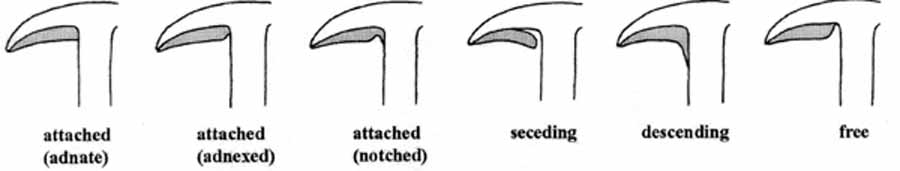
\includegraphics[width=0.5\textwidth]{plot/graphic/gill attachment.jpg}}
        \subfloat[Gill spacing.]{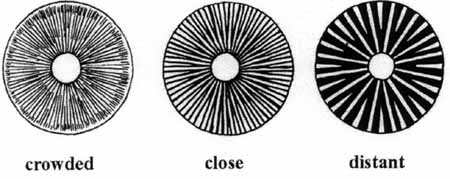
\includegraphics[width=0.5\textwidth]{plot/graphic/gill spacing.jpg}} \\
        \subfloat[Stalk root.]{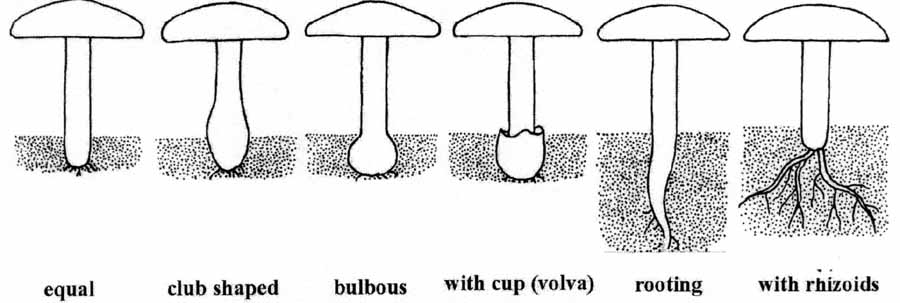
\includegraphics[width=0.5\textwidth]{plot/graphic/stalk root.jpg}}
        \subfloat[Ring type.]{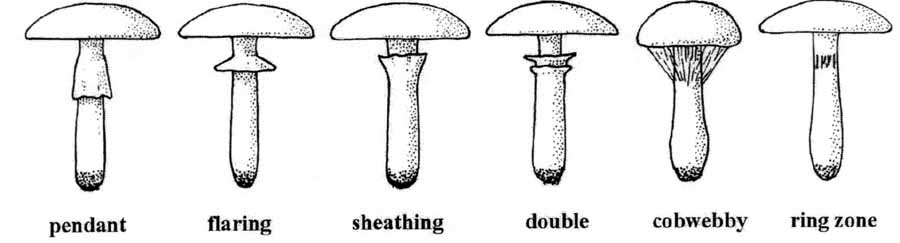
\includegraphics[width=0.5\textwidth]{plot/graphic/ring type.jpg}} \\
        \caption{Some mushroom features included in the dataset. [2]}
        \label{fig:graphic1}
    \end{figure*}

    \subsection{Characteristics}
    \subsubsection{Target Features}
    In Table I, we see that the classification type is binary, where a mushroom is determined to be either poisonous or edible. Edible mushrooms are fungi that humans can safely eat as food. Poisonous mushrooms, on the other hand, are fungi that can be toxic and harmful if ingested, potentially leading to illness or death.
    \begin{table}[htbp]
        \centering
        \caption{\\ TARGET} 
        \begin{tabular}{cc} \toprule
                \textbf{Feature} & \textbf{Values} \\
            \midrule
                \multirow{1}*{Class}
                    & edible, poisonous \\
            \bottomrule
        \end{tabular}
    \end{table}

    \subsubsection{Cap Features}
    Moreover, Table II shows the various cap features of mushrooms, where the cap is considered the mushroom's uppermost body structure and often looks like an umbrella. The cap shape is how this upper portion is formed and the cap surface is the type of structure found at the top of the mushroom.
    \begin{table}[htbp]
        \centering
        \caption{\\ CAP}
        \begin{tabular}{cc} \toprule
                \textbf{Feature} & \textbf{Values} \\
            \midrule
                \multirow{2}*{Shape}
                    & bell, conical, convex, \\
                    & flat, knobbed, sunken  \\
            \midrule
                \multirow{1}*{Surface}
                    & fibrous, grooves, scaly, smooth \\
            \midrule
                \multirow{3}*{Color}
                    & brown, buff, cinnamon, gray, \\
                    & green, pink, purple, red,    \\
                    & white, yellow                \\
            \bottomrule
        \end{tabular}
    \end{table}

    \subsubsection{Gill Features}
    Table III depicts the different gill features in mushrooms, a major characteristic that is located underneath the mushroom cap. The gill attachment is the way the gills grow on the mushroom's stem, the gill spacing is the arrangement of the gills and their distribution, and the gill size is the width of the gills—where "broad" indicates thickness and "narrow" indicates thinness.
    \begin{table}[htbp]
        \centering
        \caption{\\ GILL}
        \begin{tabular}{cc} \toprule
                \textbf{Feature} & \textbf{Values} \\
            \midrule
                \multirow{2}*{Attachment}
                    & attached, descending, \\ 
                    & free, notched \\
            \midrule
                \multirow{1}*{Spacing}
                    & close, crowded, distant \\
            \midrule
                \multirow{1}*{Size}
                    & broad, narrow \\
            \midrule
                \multirow{3}*{Color}
                    & black, brown, buff, chocolate, \\
                    & gray, green, orange, pink,     \\
                    & purple, red, white, yellow     \\
            \bottomrule
        \end{tabular}
    \end{table}

    \subsubsection{Stalk Features}
    Table IV illustrates a mushroom's possible stalk features. The stalk shape is the shape of the mushroom's stem that holds the cap above the ground. Some mushrooms possess stalks with a thicker base ("enlarged") and others possess stalks that start to thin from cap to base ("tapering"). Additionally, the stalk root is the lower part of the stem that attaches to or makes contact with a substrate. The stalk surface is the structure above or below the mushroom's ring, and the stalk color is the color of the stalk above or below the mushroom's ring.
    \begin{table}[htbp]
        \centering
        \caption{\\ STALK}
        \begin{tabular}{cc} \toprule
                \textbf{Feature} & \textbf{Values} \\
            \midrule
                \multirow{1}{5em}{Shape}
                    & enlarging, tapering  \\
            \midrule
                \multirow{2}{5em}{Root}
                    & bulbous, club, cup, equal,   \\
                    & rhizomorphs, rooted, missing \\
            \midrule
                \multirow{3}{5em}{Surface above/below ring}
                    & \\
                    & fibrous, scaly, silky, smooth \\
                    & \\
            \midrule
                \multirow{3}{5em}{Color above/below ring}
                    & brown, buff, cinnamon,   \\
                    & gray, orange, pink, red, \\
                    & white, yellow            \\
            \bottomrule
        \end{tabular}
    \end{table}
    
    \subsubsection{Veil Features}
    Furthermore, Table V portrays the veil features of the mushroom, where the veil type is the kind of veil membrane the mushroom has, and the veil color is simply the color of the mushroom's veil.
    \begin{table}[htbp]
        \centering  
        \caption{\\ VEIL}
        \begin{tabular}{cc} \toprule
                \textbf{Feature} & \textbf{Values} \\
            \midrule
                \multirow{1}*{Type}
                    & partial, universal \\
            \midrule
                \multirow{1}*{Color}
                    & brown, orange, white, yellow \\
            \bottomrule
        \end{tabular}
    \end{table}

    \subsubsection{Ring Features}
    Table VI outlines the potential ring features a mushroom can have, where the rings are tissue-like structures that surround the stalk of certain mushrooms. The ring number is the number of rings a mushroom has on the stalk, and the ring type refers to the type of structure that the ring possesses.
    \begin{table}[htbp]
        \centering 
        \caption{\\ RING}
        \begin{tabular}{c c}
            \toprule
                \textbf{Feature} & \textbf{Values} \\
            \midrule
                \multirow{1}*{Number}
                    & none, one, two \\
            \midrule
                \multirow{3}*{Type}
                    & cobwebby, evanescent,    \\
                    & flaring, large, none,    \\
                    & pendant, sheathing, zone \\
            \bottomrule
        \end{tabular}
    \end{table}

    \subsubsection{Miscellaneous Features}
    Finally, Table VII describes numerous characteristics that do not fall under a grouping of related features. We refer to these as miscellaneous features. The odor of a mushroom is the aroma that it emits, ranging from foul or pungent to earthy and pleasant. The spore print color is the color of the spore deposit left by a mushroom when it discharges mature spores. The population feature describes the distribution of mushrooms within a particular area, where "several" means that there are multiple individual species, "solitary" means that are only one species, "scattered" means that mushrooms are scattered throughout the area, and "clustered" means that mushrooms in the area grow in groups or colonies.
    \begin{table}[htbp]
        \centering 
        \caption{\\ MISCELLANEOUS}
        \begin{tabular}{c c}
            \toprule
                \textbf{Feature} & \textbf{Value} \\
            \midrule
                \multirow{1}*{Bruises}
                    & yes, no \\
            \midrule
                \multirow{3}*{Odor}
                    & almond, anise, creosote,  \\
                    & fishy, foul, musty, none, \\
                    & pungent, spicy            \\
            \midrule
                \multirow{3}*{Spore print color}
                    & black, brown, buff, chocolate, \\
                    & green, orange, purple,         \\
                    & white, yellow                  \\
            \midrule
                \multirow{2}*{Population}
                    & abundant, clustered, numerous, \\
                    & scattered, several, solitary   \\
            \midrule
                \multirow{2}*{Habitat}
                    & grasses, leaves, meadows,  \\
                    & paths, urban, waste, woods \\
            \bottomrule
        \end{tabular}
    \end{table}

\section{Exploratory Data Analysis}
    \subsection{Observations}
    % Figure 2: Class features
    \begin{figure*}[htbp]
        \centering
        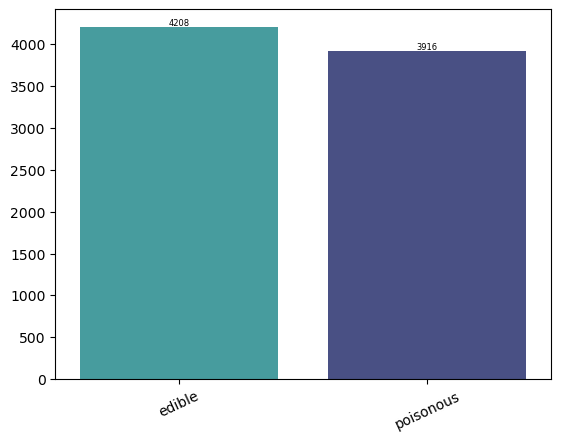
\includegraphics[width=0.6\textwidth]{plot/count/class count.png}
        \caption{Count plot of edible and poisonous mushrooms.}
        \label{fig:plot2}
    \end{figure*}
    For dataset analysis and understanding, we imported our data as a Pandas dataframe in a collaborative Jupyter notebook and dissected it with several functions to help illustrate any significant details. The original data values were all in character format, such as the categories for the "class" feature, where each entry contained either "p" for poisonous or "e" for edible. This feature was determined to be the classifier, where the target variable is "poisonous". Regardless, it was difficult to interpret the dataset with character values alone, so we reformatted them by mapping each character to its full string name. This helped us view the dataset from a more verbose and clarified perspective.
   
    Overall, the dataset consists of 8,124 rows and 23 columns. As shown in Fig. 2, the target class has a roughly balanced distribution, where 51.8\% of the mushrooms are edible and 48.2\% are poisonous. It is important to note that every column is categorical (i.e., in character format), where techniques such as label encoding and one-hot encoding must be applied to transform the data into a usable, numerical format. From this, we gathered statistics such as percentage breakdowns of each column to influence what variables we should keep or remove.

    \subsection{Feature Selection}
    % Figure 3: Dropped features
    \begin{figure*}[htbp]
        \centering
        \subfloat[Gill attachment.]{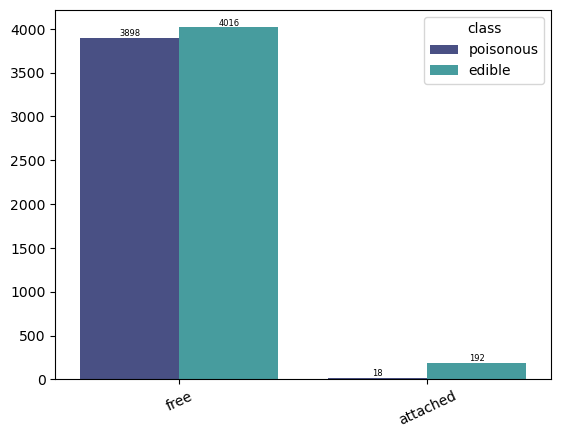
\includegraphics[width=0.45\textwidth]{plot/count/gill attachment count.png}}
        \subfloat[Stalk shape.]{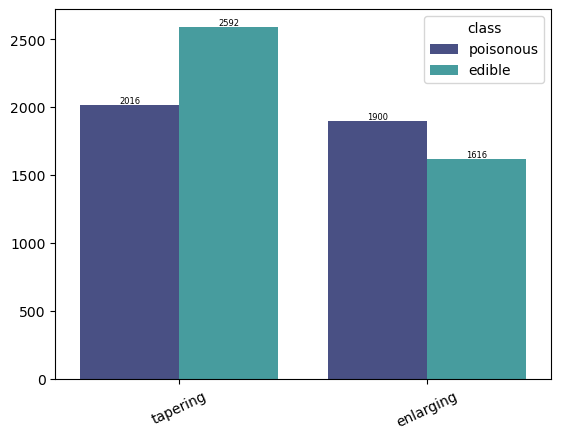
\includegraphics[width=0.45\textwidth]{plot/count/stalk shape count.png}} \\
        \subfloat[Stalk root.]{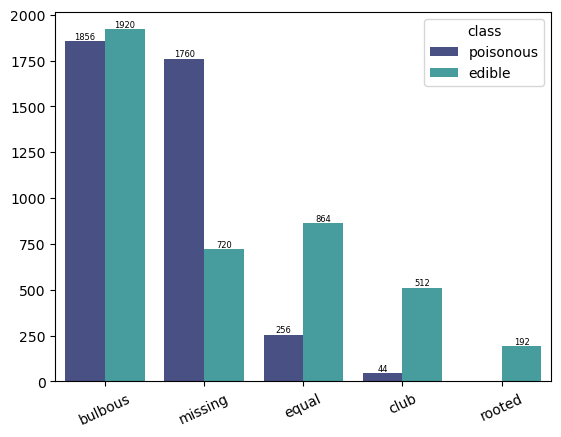
\includegraphics[width=0.45\textwidth]{plot/count/stalk root count.png}}
        \subfloat[Stalk surface below ring.]{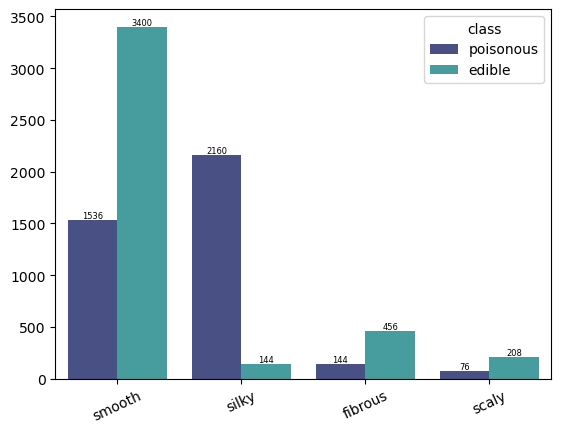
\includegraphics[width=0.45\textwidth]{plot/count/stalk surface below ring count.png}}
        \label{fig:plot3}
    \end{figure*}
    
    \begin{figure*}[htbp] \ContinuedFloat
        \centering
        \subfloat[Stalk color below ring.]{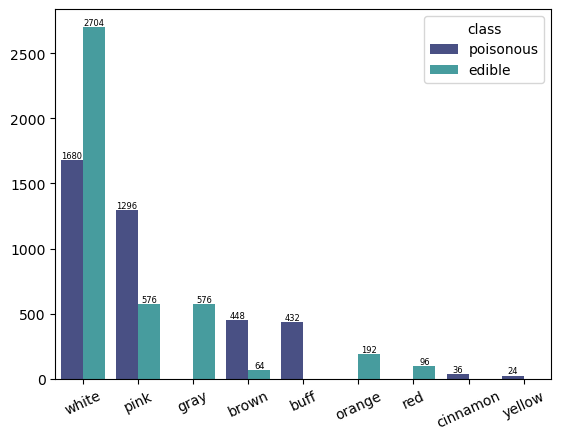
\includegraphics[width=0.45\textwidth]{plot/count/stalk color below ring count.png}}
        \subfloat[Veil type.]{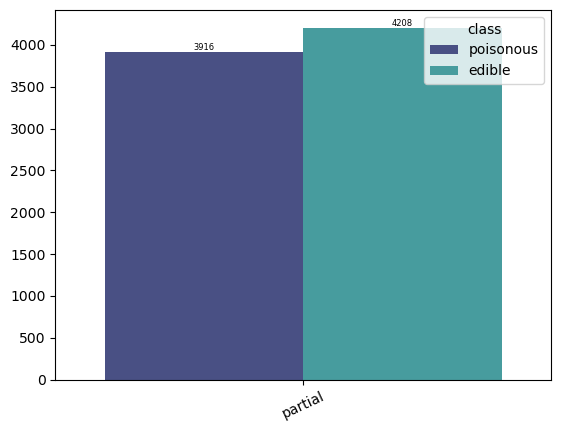
\includegraphics[width=0.45\textwidth]{plot/count/veil type count.png}} \\
        \subfloat[Veil color.]{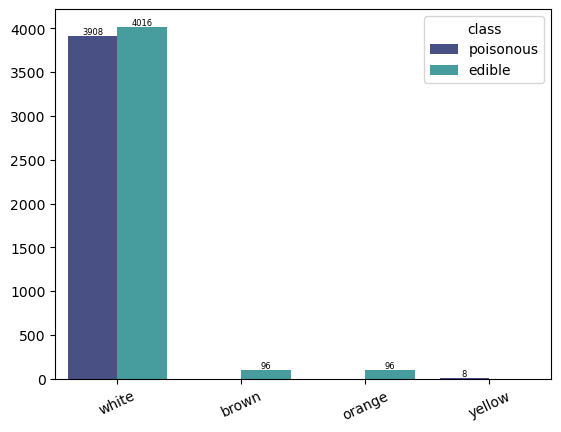
\includegraphics[width=0.45\textwidth]{plot/count/veil color count.png}} 
        \subfloat[Ring number.]{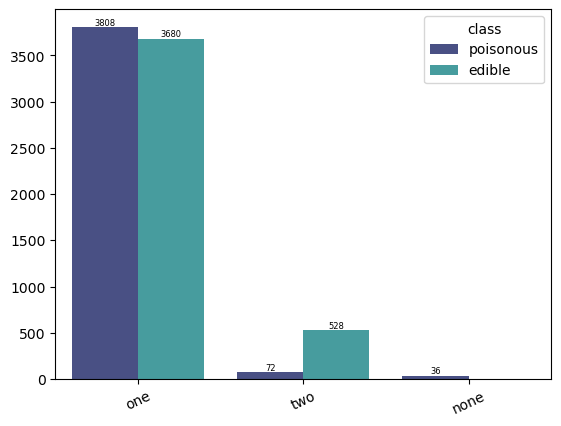
\includegraphics[width=0.45\textwidth]{plot/count/ring number count.png}}
        \caption{Count plots of insignificant features that were dropped from training.}
    \end{figure*}

    In Fig. 3a, we discovered that the mushroom dataset has a large majority of samples that have free gill attachments (97.42\%). The veil type feature in Fig. 3f was the largest indicator of this, where 100\% of the samples were all one type ("partial"). This trend can also be observed in Fig. 3h, where 92.17\% of mushrooms have one ring. The veil color, shown in Fig. 3g, also had a similar case, where 97.54\% of the mushrooms have white veil colors and 2.46\% make up the others. Ultimately, the skewed nature of these distributions signifies variables that do not provide enough unique information that can effectively train our model.

    As depicted in Fig. 3b, we also observed that 56.72\% of the mushrooms have tapering stalk shapes while 43.28\% have enlarging stalk shapes. With this relatively even distribution, we can also see that there is an insignificant difference between the poisonous and edible mushrooms for each value. There were also missing data values that we had to consider, as seen in Fig. 3c. 30.53\% of the mushrooms had an unknown stalk root, which indicated inconclusive data that we decided to ignore during model training. Additionally, for Fig. 3d and Fig. 3e, we noticed that the stalk surface and the stalk color below the ring had closely similar distributions to their above-the-ring counterparts. As a result, such features were eliminated from the dataset to ensure that our model utilizes the most useful information.

\section{Proposed Methodology}
    \begin{table}[htbp]
        \centering  
        \caption{\\ CLASSIFIERS}
        \begin{tabular}{cc} \toprule
            \textbf{Model} \\
            \midrule
                Logistic Regression \\
            \midrule
                Perceptron Learning \\
            \midrule
                Gaussian Naive Bayes \\
            \midrule
                Multinomial Naive Bayes \\
            \midrule
                Categorical Naive Bayes \\
            \midrule
                Dummy Classifier \\
            \midrule
                Decision Tree \\
            \midrule
                Random Forest \\
            \bottomrule
        \end{tabular}
    \end{table}

    \subsection{Classification Models}
    Given the variety of different models that can be applied to this dataset, we decided to train with the classifiers listed in Table VIII and compile performance metrics for each model to help evaluate their robustness. These models were discovered through background research and imported through the \texttt{scikit-learn} library, which also contained several other classifiers that we could have included in our experiments. However, to stay within the scope of what was taught in class, we limited training on select models that were covered in the lectures. 
    
        \subsubsection{Logistic Regression}
        Logistic Regression is a linear model commonly used for binary classification problems. It estimates the probability that a given input belongs to a particular category. This fits within our dataset because we are faced with the binary task of determining edibility, where 0 is encoded as edible and 1 is encoded as poisonous.

        \subsubsection{Perceptron Learning}
        Perceptron Learning is a type of linear classifier and is one of the simplest artificial neural networks. It is suitable for binary classification problems, particularly for linearly separable data.

        \subsubsection{Naive Bayes}
        Naive Bayes classifiers apply Bayes' theorem with strong (naive) independence assumptions between features. There are several types depending on the distribution of the data.
            \paragraph{Gaussian}
            Gaussian Naive Bayes is a variant of the Naive Bayes classifier that assumes the features follow a Gaussian (normal) distribution. It's fast, simple, and performs well with smaller datasets.

            \paragraph{Multinomial}
            Multinomial Naive Bayes is used for classification with discrete features and is effective for high-dimensional data. 

            \paragraph{Categorical}
            Categorical Naive Bayes is a variant that is highly suitable for problems where features are categorical rather than continuous. This is the type of classifier that fits most with the nature of our dataset. However, like every Naive Bayes variant, it assumes that features are independent, which may not be realistic for all datasets.

            Although the Gaussian and Multinomial variants do not particularly follow the distribution of our dataset, it is important to include them in our model evaluations for comparison purposes.

        \subsubsection{Dummy Classifier}
        The Dummy Classifier is a simple baseline classifier that makes predictions based on simple rules, such as predicting the most frequent class or making random predictions. Since it does not provide meaningful predictions, it is only used to compare the performance of the other classifiers.

        \subsubsection{Decision Tree}
        The Decision Tree Classifier uses a tree-like model of decisions and their possible consequences. It splits the data into subsets based on the value of input features and can handle both numerical and categorical data.

        \subsubsection{Random Forest}
        The Random Forest Classifier is an ensemble learning method that constructs multiple decision trees during training. By averaging multiple trees, it reduces overfitting and improves accuracy. It is suitable for a variety of classification problems and handles missing values well.
    
    \subsection{Preprocessing}
    To prepare the model for training, data preprocessing was conducted to allow the machine learning algorithms to effectively utilize the input information. The data was split into their corresponding train and test sets, with X\_train and X\_test for the dependent variables and y\_train and y\_test for the target class. Label encoding and one-hot encoding were used for the y and X variables, respectively. With only two distinct values between the classes, the use of label encoding for the target feature is suitable for defining an intrinsic order within a few categories, where 0 stands for edible and 1 stands for poisonous. In this case, more meaning is assigned to the "poisonous" class, which corresponds with our model's purpose in determining whether or not a mushroom is dangerous to eat. Moreover, since we are dealing with categorical data that is nominal (lacks inherent order) for the dependent variables, one-hot encoding transforms this information into a numerical format that can be used in model training.

    \subsection{Metrics}
    With that, several performance metrics are measured for each model that grant us insight into how well the classifier performs on our dataset. To do this, a variety of scores for each model are stored in a metrics dataframe for us to review. Many of these scores were calculated with the help of the \texttt{scikit-learn} module.

    \begin{figure*}[ht!]
        \centering
        \subfloat[Accuracy.]{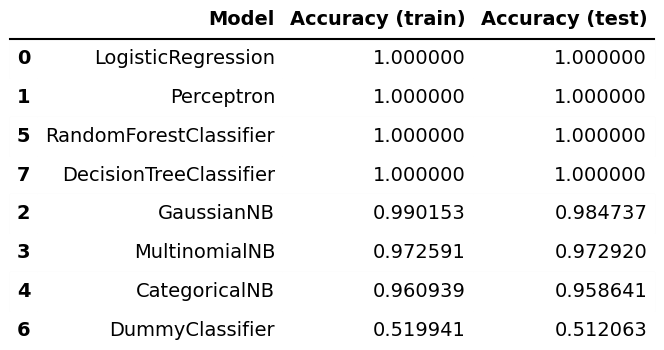
\includegraphics[width=0.45\textwidth]{plot/table/accuracy.png}}
        \subfloat[Precision.]{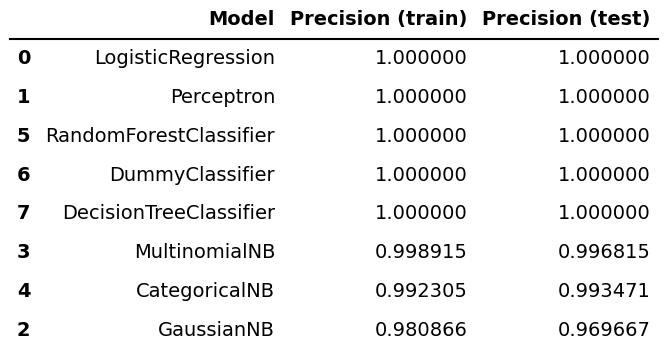
\includegraphics[width=0.45\textwidth]{plot/table/precision.png}} \\
        \subfloat[Recall.]{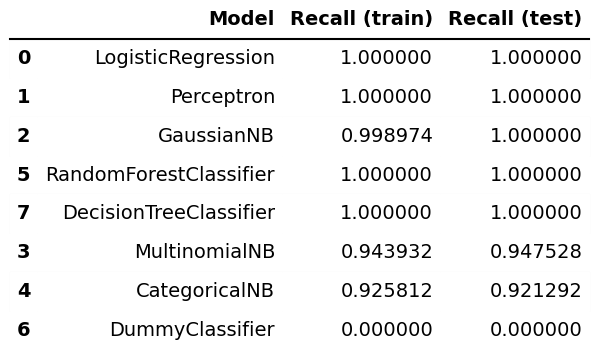
\includegraphics[width=0.45\textwidth]{plot/table/recall.png}}
        \subfloat[F1 score.]{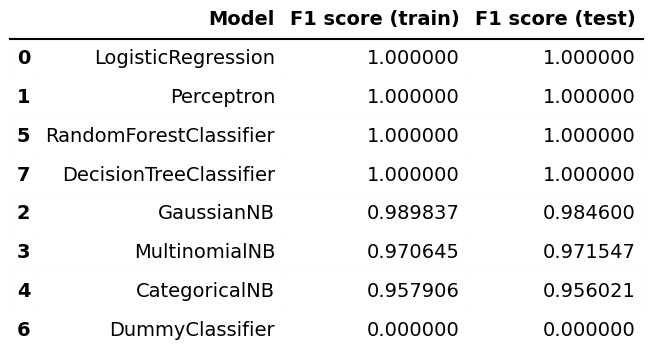
\includegraphics[width=0.45\textwidth]{plot/table/f1.png}}
        \caption{Tables of performance metrics sorted in ascending order according to the test measure.}
        \label{fig:graphic2}
    \end{figure*}

    \subsubsection{Accuracy}
    Classification accuracy is a commonly used metric that measures the proportion of correct predictions made by a model out of the total predictions made. It is defined as the ratio of the number of correctly classified instances (both true positives and true negatives) to the total number of instances. In our source code, we iterate through ground truth values and compare them with generated predictions to produce an accuracy score.

    \begin{equation}
        \text{Accuracy} = \frac{\text{TP} + \text{TN}}{\text{TP} + \text{TN} + \text{FP} + \text{FN}}\label{eq1}
    \end{equation}
    
    Accuracy can be misleading in cases of imbalanced datasets, where the number of instances in one class significantly outweighs the number of instances in another class. In our case, the number of instances in each of our target classes has a nearly even split. Overall, accuracy is a basic yet important metric that provides a direct measure of a machine learning model's performance by indicating how often the model's predictions are correct. 

    \subsubsection{Precision}
    Precision is defined as the ratio of true positive predictions (correctly predicted positive cases) to the total number of positive predictions made by the model (both true positives and false positives). In other words, it is a measure of the accuracy of the positive predictions that are made by a model. 
    \begin{equation}
        \text{Precision} = \frac{\text{TP}}{\text{TP} + \text{FP}}\label{eq2}
    \end{equation}
    A high precision means that when the model predicts a positive class, it is very likely to be correct. Precision is particularly useful in scenarios where the cost of false positives is high. For instance, in the case of our classification problem, it can be a matter of life or death if a poisonous mushroom is accidentally ingested.
    
    \subsubsection{Recall}
    Also known as sensitivity or true positive rate, recall is a measure of a model's ability to correctly identify all relevant instances within a dataset. Specifically, it quantifies the proportion of actual positive cases that are correctly identified by the model.
    \begin{equation}
        \text{Recall} = \frac{\text{TP}}{\text{TP} + \text{FN}}\label{eq3}
    \end{equation}
    A higher value indicates that the model is more effective at identifying positive instances. Recall is particularly important in situations where missing positive cases is more critical than incorrectly identifying negatives.
    
    \subsubsection{F1 score}
    The F1 score is a widely known metric used in machine learning for evaluating the performance of classification models, especially in binary classification tasks. The F1 score is the harmonic mean of precision and recall and balances both metrics, making it useful for evaluating the overall performance of a classification model.
    \begin{equation}
        \text{F1 score} = 2 \times \frac{\text{Precision} \times \text{Recall}}{\text{Precision} + \text{Recall}}\label{eq4}
    \end{equation}

\section{Model Evaluation}
    \begin{figure*}[htbp]
        \centering
        \begin{minipage}{0.5\textwidth}
            \centering
            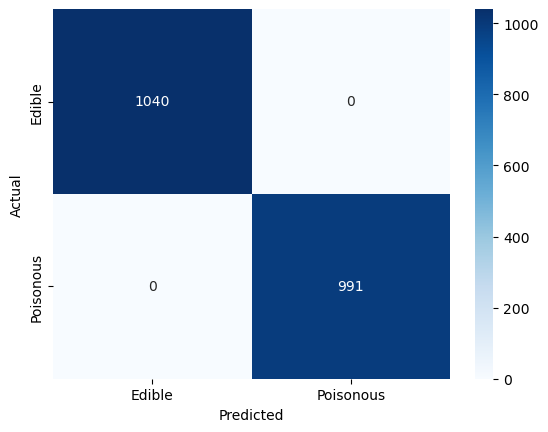
\includegraphics[width=0.75\linewidth]{plot/matrix/randomforest.png}
            \caption{Confusion matrix for Random Forest.}
            \label{fig:plot5}
        \end{minipage}%
        \begin{minipage}{0.5\textwidth}
            \centering
            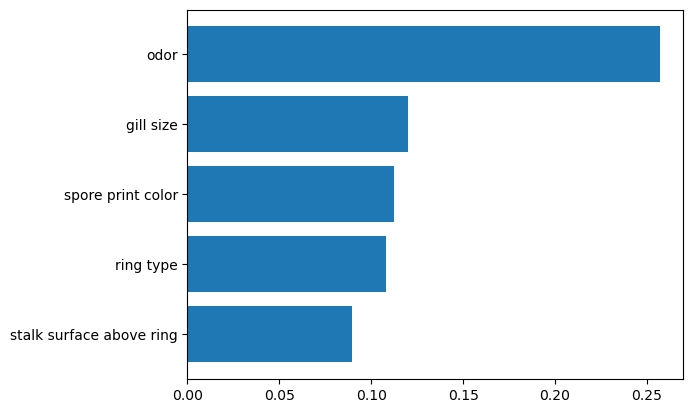
\includegraphics[width=1\linewidth]{plot/count/rf_importance.png}
            \caption{Random Forest's most important features.}
            \label{fig:plot6}
        \end{minipage}
    \end{figure*}
    
    \begin{figure*}[htbp]
        \centering
        \subfloat[Odor.]{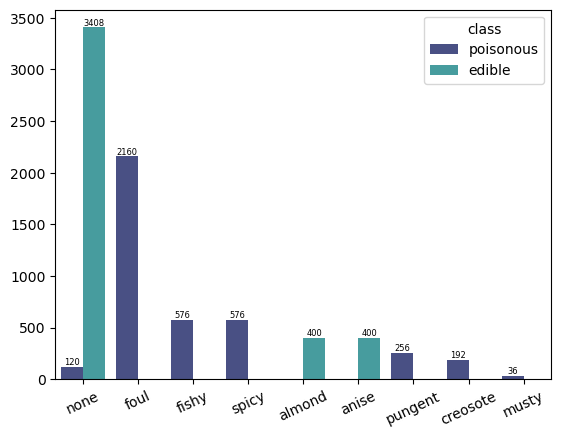
\includegraphics[width=0.45\textwidth]{plot/count/odor count.png}}
        \subfloat[Gill size.]{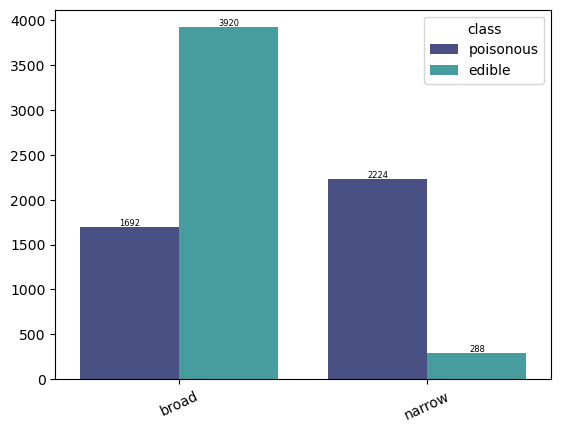
\includegraphics[width=0.45\textwidth]{plot/count/gill size count.png}}
    \end{figure*}

    \subsection{Experimental Results}
    Evaluating machine learning models is a critical step in ensuring their effectiveness, reliability, and validity. According to Fig. 4, several of our models were reported to have 100\% accuracy, precision, recall, and F1 scores by our metrics dataframe. While this may initially indicate a perfect performance, it raises the question of whether there was potential overfitting with the data. To further explore this, we took measures from both training and testing sets and included them in our tables. A great difference in performance between the training and testing sets possibly indicates an overfit. However, since the two score columns tend to closely or completely match each other, this does not seem to be the case.
    
    The top 5 models that performed well include Logistic Regression, Perceptron, Gaussian Naive Bayes, Decision Tree, and Random Forest. Since Logistic Regression primarily deals with binary classification tasks, it turned out to be a great model for our mushroom problem. Perceptron Learning was also suitable with its linear approach. The Decision Tree and Random Forest classifiers exhibited top scores as well. Although Decision Trees can be more susceptible to overfitting, Random Forest acts as an ensemble of decision trees that merges them to produce more accurate and stable predictions. 

    On the other hand, Gaussian Naive Bayes outperformed both the Multinomial and Categorical variants on every level. Theoretically, Categorical Naive Bayes should have performed better due to the nature of our dataset.
    However, since these features were transformed through encoding, we ended up benefiting the performance of Gaussian Naive Bayes while hindering the performance of the Categorical variant. Even after explicitly converting the feature data types during data formatting, it seems that the Categorical variant was not insensitive to feature encoding. 

    As for the overall performance of the Naive Bayes models (with scores below 100\%), it is important to remember that these algorithms operate with the assumption of independent features, which is not strictly the case for our variables. For instance, mushrooms with certain cap colors might be more prone to bruising, or bruising may change the apparent color of the cap. The type of habitat where a mushroom grows (woods, grass, etc.) can also be related to the population size. For example, mushrooms that grow in woods might be found in smaller populations compared to those growing in open fields.

    Finally, the Dummy Classifier serves as a reference point to understand if a more sophisticated model is actually learning meaningful patterns from the data, or if it is just performing at the level of a naive strategy. As we can see from the accuracy table in Fig. 4a, the Dummy Classifier correctly classifies a poisonous mushroom approximately 50\% of the time.

    \begin{figure*}[htbp] \ContinuedFloat
        \subfloat[Spore print color.]{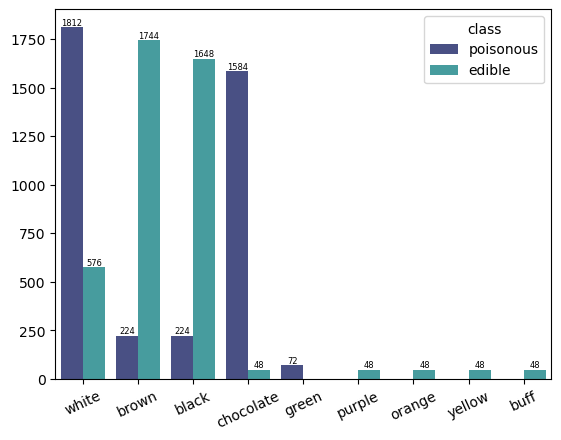
\includegraphics[width=0.33\textwidth]{plot/count/spore print color count.png}}
        \subfloat[Ring type.]{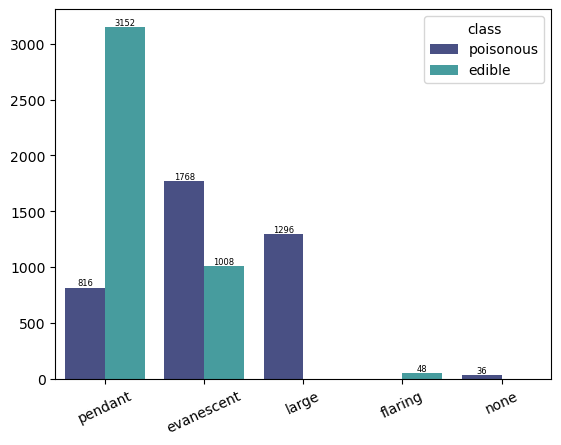
\includegraphics[width=0.33\textwidth]{plot/count/ring type count.png}}
        \subfloat[Stalk surface above ring.]{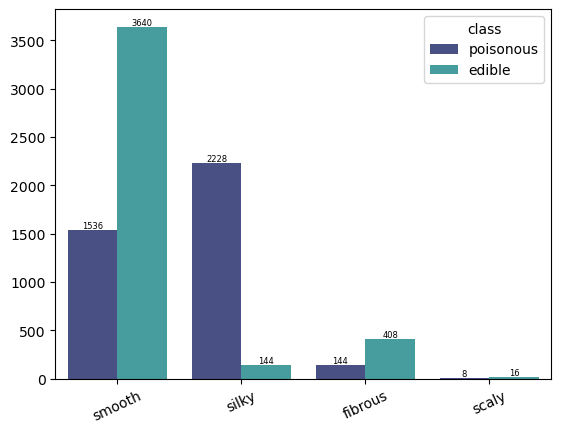
\includegraphics[width=0.33\textwidth]{plot/count/stalk surface above ring count.png}}
        \caption{Count plots of the top features in descending order.}
        \label{fig:graphic3}  
    \end{figure*}

    \subsection{Confusion Matrix}
    To help identify any patterns of misclassification, a confusion matrix was used to provide a visual summary of the predictions compared to the ground truths. With a 100\% accuracy rate, the confusion matrix for the top models (Linear Regression, Perceptron, Decision Tree, and Random Forest) is shown in Fig. 5. For further exploration into our experimental results and their implications as a whole, we decided to focus on the Random Forest model.

    \subsection{Feature Importance}
    Included in the \texttt{scikit-learn} library's Random Forest Classifier is gini importance, a measure used to evaluate the significance of features in decision tree models. Also known as Mean Decrease in Impurity (MDI), it helps in understanding which features contribute the most to the prediction accuracy of the model. With Fig. 6, we can see the Random Forest model's report of the top 5 most important features: odor, gill size, spore print color, ring type, and stalk surface above the ring.

\section{Discussion and Conclusion}
    Based on the insights gained from the model training and evaluation, certain features stand out as strong indicators of whether a mushroom is edible or poisonous. The most important feature determined by the Random Forest model is odor. According to Fig. 7a, mushrooms without any discernible odor are more likely to be edible, while those with a foul smell are more likely to be poisonous. The width of the gills also plays a significant role. In Fig. 7b, Mushrooms with narrow gills tend to be more poisonous, while those with broad gills are predominantly edible. However, it's worth noting that even broad-gilled mushrooms may carry some risk of toxicity. For Fig. 7c, mushrooms leaving white or chocolate-colored spore prints are more likely to be poisonous, whereas those leaving brown or black prints are generally safer to consume. Show in Fig. 7d, mushrooms with a pendant ring are more likely to be edible, while those with an evanescent (disappearing) or large ring are more likely to be poisonous. Finally, in Fig. 7e, mushrooms with a silky stalk surface above the ring are typically poisonous, whereas those with a smooth surface are more likely to be edible.

    In this project, we explored the application of machine learning models for classifying the edibility of wild mushrooms. Among the classifiers tested, decision trees and random forests emerged as the most effective models due to their high accuracy, robustness, and interpretability. Overall, this study demonstrates that machine learning can be a powerful tool in mycology for identifying potentially dangerous mushrooms, highlighting the importance of leveraging computational methods for enhancing food safety practices. The findings of this report pave the way for developing reliable, automated systems for mushroom edibility classification, contributing to both scientific research and practical applications in the field. Future work could involve expanding the dataset, exploring additional features, and integrating advanced techniques like deep learning to further enhance classification performance.
    
    \begin{table}[htbp!]
        \centering
        \caption*{\\ PROJECT ROADMAP }
        https://github.com/sutibn/ECS171GroupProject
        \begin{tabular}{cc} \toprule
                \textbf{Goal} & \textbf{Date} \\
            \midrule
                \multirow{1}*{Dataset selection and understanding}
                    & 4/19 \\
            \midrule
                \multirow{1}*{Background study/literature review}
                    & 4/26 \\
            \midrule
                \multirow{1}*{Exploratory data analysis}
                    & 5/3 \\
            \midrule
                \multirow{1}*{Develop and evaluate prediction models}
                    & 5/17 \\
             \midrule
                \multirow{1}*{Record observations and write the report}
                    & 5/24 \\
             \midrule
                \multirow{1}*{Develop HTML web page to deploy the model}
                    & 5/31 \\
            \midrule
                \multirow{1}*{Finish the written report and the model demo}
                    & 6/7 \\
            \bottomrule
        \end{tabular}
    \end{table}

% References (bib/sources.bib to add/change entries)
\onecolumn
\nocite{*}
\bibliographystyle{bib/IEEEtran}
\bibliography{bib/sources}
\end{document}
